\documentclass[12pt, a4paper]{report}   % list options between brackets
\usepackage{setspace}
\usepackage{graphicx}
\graphicspath{../content/}



\begin{document}

\begin{center}

% Upper part of the page
\textsc{\large University of Sussex}\\[1.5cm]
\textsc{Final year project}\\[2cm]

% Title
\begin{spacing}{2.5}
{\Large \bfseries Estimating personal energy expenditure \\ with location data}\\[5 cm]
\end{spacing}
\end{center}
\vfill

% Author and supervisor
\begin{spacing}{1.5}
\begin{tabular}{l}
Student Name: Vladimir Hartmann \\
Degree program: BSc Computer Science \\
Department: School of Informatics \\
Candidate Number: 52665 \\
Project Supervisor: Dr. Martin Berger \\
Date of Submission: {\today}
\end{tabular}
\end{spacing}
\thispagestyle{empty}


% Abstract
\begin{abstract}
  A brief introduction ...
\end{abstract}

% Table of content
\tableofcontents
\thispagestyle{empty}

% Introduction
\clearpage
\pagenumbering{arabic}
\chapter{Introduction}

\section{Motivation}
Modern society is putting unsustainable demands on personal wellbeing as well as the wellbeing of the planet. Pervasive sedentary lifestyle has been creating many health conditions while excess in energy consumption has had adverse effects on our ecosystem. There is a clear connection between personal and planetary wellbeing and actions that help to improve our own health often have a positive effect on our environment. Location data such as GPS tracking can be utilised to address both issues. As it is most frequently collected piece of contextual data in computing, it can be applied to many healthcare applications. This technique offers a number of improvements over traditional methods, which involve carrying a dedicated accelerometer device.

\section{Current systems}
Tracking people’s movement has been known for some time now. Romans used odometer calibrated to steps, although technically not a step counter, the idea was similar. Leonardo Da Vinci designed a mechanical pedometer, which was used for civil and military purposes. Most of the movements tracking solution on the market today make use accelerometer, which is a device able to monitor any movement in X, Y and Z coordinates. This approach however requires wearing a special device, which might not me convenient. It is also not accurate in many cases (user can cheat by only moving the device in certain way to mimic the actual walking/running).
Proposed approach in this project uses mainly GPS data to track users movement. This can be supported (with project extensions) by accelerometer data and data obtained from signals of the heartbeat. All three technologies combined can produce very accurate and reliable system.

\section{About this project}

\section{Aims and objectives}
Aims:
\begin{itemize}
\item Estimate personal energy expenditure and provide healthy recommendations for personal and planetary wellbeing.
\end{itemize}
Objectives:
\begin{enumerate}
\item (primary) Design and develop the Personal Energy Meter (PEM), an iPhone application
\item (primary) Design and develop an Interactive Dynamic Website
\item (extension) Ensure that both systems are reliable and accurate
\item (extension) Validated with real biomedical measurements
\item (extension) Extended functionality for better user experience
\end{enumerate}
For details on objectives see Requirements Analysis (Project after negotiation) section

% Background
\chapter{Background}

% Requirements
\chapter{Requirements Analysis}

\section{Requirements discovery}
Requirements discovery has been carried out on three individuals. The project supervisor/main customer Martin and two friends of mine Tim and Richard. The requirements are very vague and high-level but refined throughout the stages of the Requirement Analysis.

\subsection{Collected scenarios}
\subsubsection*{Scenario 1}
Martin has a busy lifestyle in which time to rest and sleep is very precious. Therefore he would like to find a way of measuring and controlling the amount of energy he uses doing certain activities such as walking, running, cycling, working out in the gym or climbing stairs. As he is also very aware of the carbon footprint on the environment he would be interested in how much he could eliminate the emissions by changing his forms of transport.

\subsubsection*{Scenario 2}
Tim spends lots of hours in an office doing a sedentary job. To preserve his wellbeing he wants to know each day/week whether he had enough recommended physical activity. He would like to get accurate calorie expenditure results with healthy advices and recommendations directly on his iPhone or access it online via web page where he can log in, see all the results collected, graphically displayed using charts, and access and share other people’s results to see general healthy trends.


\subsubsection*{Scenario 3}
Richard is a bodybuilder and therefore maintaining a strict workout program with enough rest each day is very important to him. As he is not a professional athlete he would appreciate some conventional way of keeping track of his calorie expenditure via heartbeat pulses while he works out in the gym. As a result, he would like to obtain very accurate data from which he could design or improve his workout program.

\section{Requirements classification and \\ organization}
On examination of all three scenarios and after consideration of the resources available for undertaking the project, following decisions have been made and presented to customer at one of the formal meetings: iPhone development will be used as this device was already available. (Developing for an iPhone also brings new challenges of learning new programming language, API and interesting development methods and models to this project.)

\subsubsection*{Product functionality}

The iPhone application should have following functionalities:

	\begin{itemize}
	\item Capture, categorize and process data (GPS, sound signal, accelerometer)
	\item Calculate calories expenditure using an Energy Consumption Model
	\item Calculate a carbon footprint
	\item Graphically output the results of the calculations
	\item Give recommendations on personal and planetary wellbeing
	\end{itemize}
For accessing captured data from a computer an interactive dynamic website will be build. For the purposes of applying the knowledge of a Java language and Web Computing the website will be coded using Java EE 6 which is the industry standard for enterprise Java computing. This website should have following functionalities:
\begin{itemize}
\item Create and maintain user profiles
\item Receive and process data from the iPhone application
\item Graphically output results of calculations
\item Give recommendations on personal and planetary wellbeing
\item Share personal energy expenditure data with other users
\item Energy expenditure trends visualisation (personal, carbon footprint)
\end{itemize}
The classification and organization of the requirements discovery was a first important step of translating the high level user’s scenarios to more technical and measurable units.

\section{Requirements prioritization and \\ negotiation}
Although the classification and organization phase of the requirements discovery laid down some understandable structure to the project, which is closer to implementation than vague user scenarios, the time constraint of the project became very apparent. Negotiations with the customer therefore had to take place in order to preserve prototype and final product release dates schedule.

\subsubsection*{Objectives after negotiation}
Primary:
	\begin{itemize}
		Design and develop the Personal Energy Meter (PEM), an iPhone application that 		should 	have following functionalities:
	\end{itemize}
	\begin{itemize}
		\begin{itemize}
			\item Capture and process GPS data
			\item Calculate calories expenditure using an Energy Consumption Model
			\item Calculate a carbon footprint
			\item Graphically output results of the calculations
			\item Give recommendations on personal and planetary wellbeing
Design and develop an interactive website which should have following functionalities:
			\item Create and maintain user profiles
			\item Receive and process data from the PEM, an iPhone application
			\item Graphically output results of calculations
			\item Give recommendations on personal and planetary wellbeing
		\end{itemize}
	\end{itemize}
Extensions: 
	\begin{itemize}
		\begin{itemize}
			\item More precise GPS data processing by PEM
			\item Live GPS data categorization (walking, driving car, running, using public transport)
			\item iPhone in-built headphones microphone integration for capturing the heartbeat (for estimating energy expenditure indoors where high volume of energy can be used for example in the gym or climbing stairs)
			\item Validation of the Energy Consumption Model with real biomedical measurements
			\item Improve accuracy and reliability of capturing the GPS data
			\item Share the personal energy expenditure data with other users
			\item Energy expenditure trends visualization (personal, carbon footprint)
		\end{itemize}
	\end{itemize}
Splitting the project requirements, by negotiating with the customer, into two categories (Primary, Extensions) reduced a development overhead, which wasn’t apparent in the initial stages of formal meetings. The negotiation gave both stakeholders more clear understanding of what can be achieved within designated time of the project (or how much the customer can have for what s/he paid). The development company has however offered the customer, for keeping a good customer relations, an implementation of some or all ‘Extensions’ if time allows.

\section{Requirements Specification}
To be re-created to reflect a feedback...

% Project plan
\section{Project plan}
\subsection{Project Outline}
The goal of the project is to develop a system that can estimate users energy expenditure and advice them about their wellbeing as well as about wellbeing of the planetary environment. The main idea is to implement an iPhone application, which will be able to receive GPS data and perform live calculations of calorie burn. The basic implementation of this application requires that user performs some activity, which involves location movement.\\ \\
More advanced implementation (using the project extensions) will allow user to perform any physical activity. This means that except GPS data, the application will be able to process heartbeat signals and accelerometer data.\\ \\
The system is split into two parts, the Personal Energy Meter (PEM) which is an iPhone application and Interactive Dynamic Website (IDW). Implementation of IDW has two purposes. First, is to receive data from PEM and represent them in better graphical way using all real estate of computer monitor. Second, to demonstrate skills acquired during a course of study.

% Project schedule
\subsection{Project Schedule}
There are several important milestones for this project and each of those has several key tasks that must be performed. More information is given in the phase plan.
The main milestones for the project include:
\begin{itemize}
\item \textbf{General research} of the problem the project is concerned with and producing of the project plan overall (including the 
creation of this document as a guideline for the rest of the project, as well as being used 
as a general schedule). 

\item \textbf{Requirements Analysis}, aimed at finding all ambiguities, 
and determining exactly what the customer/user wants. This will include a decision on which 
design model to use.

\item \textbf{Design of the system}, which will help to determine how the applications will be structured given the limits and freedoms determined within the requirements Analysis phase.

\item \textbf{Implementation and Testing}, the stage in which the actual software systems
are developed, using the designs created in previous stage. Many different ways of checking that the completed applications are of a good standard and implementation is on schedule, will also by included here.

\item \textbf{Evaluation} stage will be concerned with answering the questions whether the systems implemented solved given problem, how well they solved it and how accurately the solution matches with requirements. Here will also be included material about how accurate the results from the PEM were to real biological measurements of energy expenditure.
\end{itemize}

% Phase plan
\subsection{Phase plan}
\subsubsection{General research}
\begin{enumerate}
	\item Literature reviews
		\begin{enumerate}
			\item Research materials about GPS systems
			\item Research materials about Accelerometer
			\item Research materials about human wellbeing by physical activity
			\item Research materials about human calories expenditure
			\item Research materials about iPhone development and iOS SDK
			\item Research materials about Objective-C
			\item Research materials about Java EE 6, Tomcat, GlassFish  
			\item Follow the book “Projects in Computing and Information Systems”
		\end{enumerate}
	\item Meeting with customer/user
		\begin{enumerate}
			\item Meetings with project supervisor
			\item Getting feedback on application prototypes from friends
		\end{enumerate}
	\item Write the project proposal
\end{enumerate}

% Requirements Analysis
\subsubsection{Requirements Analysis}
\begin{enumerate}
	\item Requirements discovery
		\begin{enumerate}
			\item User scenarios
			\item Customer/supervisor meetings
		\end{enumerate}
	\item Requirements classification and organization
		\begin{enumerate}
			\item Organizing and clarifying what has been gathered from customer/users
		\end{enumerate}
	\item Requirements prioritization and negotiation
		\begin{enumerate}
			\item Negotiating possible changes with customer/users and advice them on better suitable alternatives to meet the deadlines/budged
		\end{enumerate}
	\item Requirements specification
		\begin{enumerate}
			\item Clearing out ambiguities
			\item Producing a document which will act as a contract between customer and developer
		\end{enumerate}
	\item Write the interim report
\end{enumerate}

% Design
\subsubsection{Design}
\begin{enumerate}
	\item PEM (Objective-C)
		\begin{enumerate}
			\item High and low level design for Profile manager
			\item High and low level design for Login with authentication
			\item High and low level design for Database (Apple’s Core data)
			\item High and low level design for Statistics
			\item High and low level design for GPS tracking
			\item High and low level design for Live energy expenditure calculation
			\item High and low level design for Data transfer
		\end{enumerate}
	\item IDW (JavaEE)
		\begin{enumerate}
			\item High and low level design for Login with authentication
			\item High and low level design Profile view
			\item High and low level design Database (MySQL)
			\item High and low level design Statistics
		\end{enumerate}
\end{enumerate}
Subtasks of tasks above will consist of creating appropriate architectural design and UML diagrams, which will be later used in the implementation stage.

% Implementation and Testing
\subsubsection{Implementation and Testing}
The aim is to start as soon as possible without having to wait for total completion of solid software design – hence the agile development model. Modularization is used and attention is focused on some parts of the project, which will not change. In this way, implementation can start with only partial design. This strategy will be necessary in order to allow for any unforeseen complications in the design or implementation.
\begin{enumerate}
	\item Set up version control in Git
	\item PEM development
		\begin{enumerate}
			\item Implement Profile manager module
			\item Implement Login with authentication module
			\item Implement Database module
			\item Implement Statistics module
			\item Implement GPS tracking module
			\item Implement Live energy expenditure calculation module
			\item Implement Data transfer module
		\end{enumerate}
		Subtasks of the PEM development tasks will consist of:
		\begin{itemize}
			\item Interpreting high and low level design diagrams in Objective-C language and trying to predict any deviations from the design.
			\item Coding the agreed design
			\item De-bugging
			\item Refactoring for better code structure
			\item Writing a test cases
		\end{itemize}
	\item IDW development
		\begin{enumerate}
			\item Implement Login with authentication module
			\item Implement Profile view module
			\item Implement Database module
			\item Implement Statistics module
		\end{enumerate}
		Subtasks of the IDW development tasks will consist of:
		\begin{itemize}
			\item Interpreting high and low level design diagrams in Java language and trying to predict any deviations from the design.
			\item Coding the agreed design
			\item De-bugging
			\item Refactoring for better code structure
			\item Writing a test cases
		\end{itemize}
\end{enumarate}

% Evaluation
\subsubsection{Evaluation}
\begin{enumerate}
	\item Evaluation of how well the systems meet customer/user requirement
		\begin{enumerate}
			\item There will be feedback received from the customer/user throughout the development process. Prototypes of the systems will be released in intervals to ensure meeting the requirements as closely as possible.
		\end{enumerate}
	\item Evaluation of how the systems are reliable
		\begin{enumerate}
			\item One of the extension features is to ensure the reliability of the PEM system by researching deep into iPhone Location Services and Accelerometer and utilizing full power of the hardware. Task of this part of evaluation will be proving the reliability of PEM in extreme conditions where two or more technologies might by interchanging in live energy expenditure monitoring mode.
		\end{enumerate}
	\item Evaluation of how the systems are accurate
		\begin{enumerate}
			\item In this part of the evaluation phase real biological results of obtained from health centers or fitness centers will be compared to those calculated by PEM. Results maybe obtained on request from staff or by measuring calorie expenditure of myself on treadmill. This is very important part to having a product, which has some value at the end of the development. Note that it is also one of the extensions and not a priority to complete project.
		\end{enumerate}
\end{enumerate}

% Time estimates
\subsection{Time estimates}
Some progress on the project has already been made in form of gathering required literature, Requirements Analysis and PEM prototype implementation. Documents produced in the Requirements Analysis phase should only change if the extensions will be implemented and they will only change in terms of adding some functionality and not changing a core specification.\\ \\
Work expected in second term should include completion of high and low level design and more usable prototypes of PEM and IDW with most of the required functionality. Time has also been allowed for writing a draft report.\\ \\
Activity-on-node diagrams below show estimates of the time to complete both PEM and IDW systems. The figures have been estimated with constraints of learning new programming language in mind.

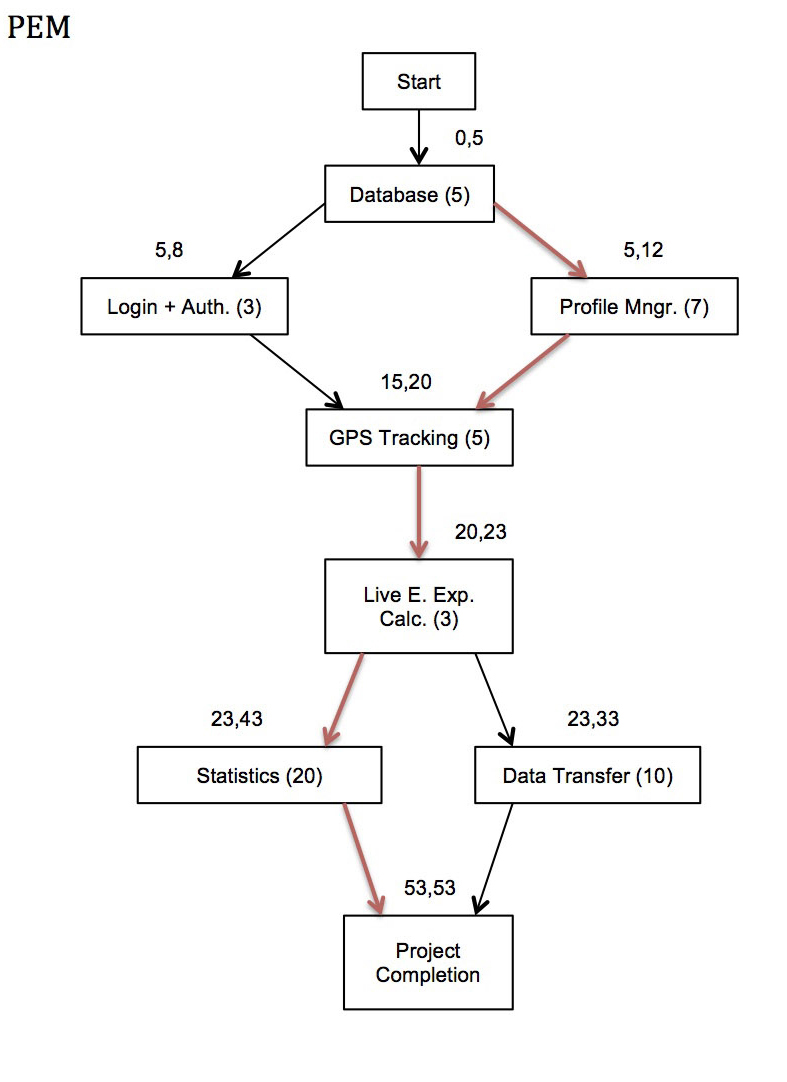
\includegraphics[width=120mm]{/content/PERTchart.jpg}

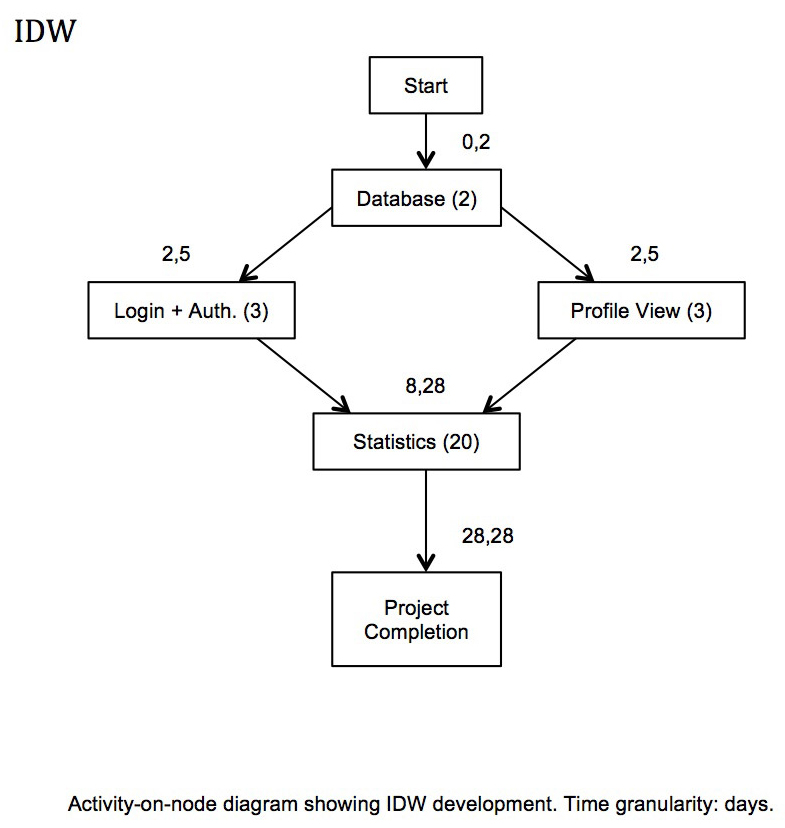
\includegraphics[width=120mm]{/content/PERTchart2.jpg}

\chapter{Design}

\chapter{Implementation and test}

\chapter{Evaluation}

\chapter{Professional Considerations}
\section{Code of Conduct}
The project raises the issue set out in section 1, subsection (a) of Code of Conduct. Implementation of Personal Energy Meter (PEM) requires use of the iPhone Location Services that gather location data of user. It must be assured that any storage or transfer of this data is secure and not leaked.\\ \\
PEM is in accordance (only if the system is used for commercial purposes) with section 1, subsections (c) and (d) of Code of Conduct, as the system will be distributed via the Apple’s App Store to which anybody can have access.\\ \\
Further issues may rise from the section 2, subsections (a) and (b) of Code of Conduct, if the systems developed would be used for commercial purposes. As part of my project is to undertake the challenge of learning new programming language and iPhone development, no full competence for these has been obtained yet. These issues have been taken into consideration however for future professional career.

\section{Code of Good Practice}
Although about 70\% of the document is closely related to this project it will be an excellent guide to ensuring that it is done correctly with highest possible quality.
Study of this document will be included as a milestone in this project.

\chapter{Conclusion}

\begin{thebibliography}{9}
  % type bibliography here
\end{thebibliography}

\chapter*{Appendices}

\end{document}






